The points that maximize the distance of the polygon will have to be anti-podal points. That implies that there exists two infinite parallel lines (support lines), each one passing by one of the two anti-podal points and not intersecting the polygon. If the above claim does not hold, and the line on point $v_k$ cuts a line of the polygon, that implies that there will be a point (where the intersecting line ends) that is more distant than $v_k$.\\

Our algorithm is based on the above property. So in order to determine the most distant points, we initialy arbitrarily choose two anti-podal points of the polygon. In order to guarantee that our initial points are anti-podal we can choose them to be two extreme points in the same direction, i.e. $y_{max}$ and $y_{min}$ (support lines are horizontal), or $x_{max}$ and $x_{min}$ (support lines are vertical). Let these points be $v_i$ and $v_j$. We keep one variable where we store the greatest distance (initialy set to zero) and two other to keep the vertices that correspond to this distance.  We create two support lines (parallel between them) one at each point. We save the distance $v_i-v_j$ as it is the so far greatest one (as well as the points $v_i$ and $v_j$), and start iterating the polygon as following:  Start rotating the support lines towards one direction (e.g. clockwise). When one of them reaches a neighboring node (when it coincides with the edge connecting to a neighboring point), we calculate the new distance and continue using as rotating center for this line the new node. At some points the lines will have exchange positions (the one that started at $v_i$ will be at $v_j$ and vice-versa). At that point the algorithm terminates, and the greatest distance is the one stored so far, since we have already iterated all the nodes (and hence all the antipodal pairs of the polygon).\\

If we consider that the calculation of distance between two points, as well as all the increasing, comparing and saving procedures can be acomplished in constant time, then the algorithm has a linear running time since we examine each node only once. The above fact holds because we stop as soon as the lines have reached the starting point of the other one that means that if we are moving in one direction (clockwise or counter-clockwise) no node will have been examined more than once.

\begin{figure}[ht]
  \centering
  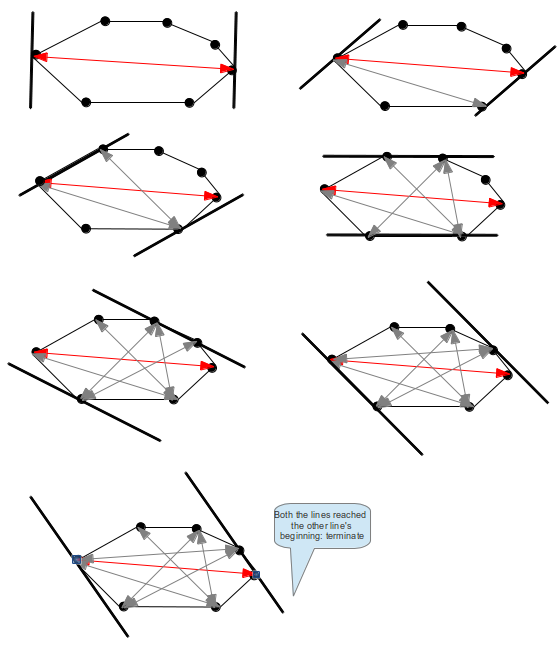
\includegraphics[width=1\textwidth]{q2}
  \caption{Execution of our algorithm}
  \label{fig:q2}
\end{figure}
\clearpage